\documentclass[tikz,border=2pt]{standalone}
\usepackage{amsmath,amssymb}
\usepackage{pgfplots}
\pgfplotsset{compat=1.18}
\usetikzlibrary{arrows.meta}
\begin{document}
% Individual risk model with n = 100 independent policies, claim probability 0.1 and fixed claim 10:
% S = 10N with N ~ Bin(100, 0.1), so S lives on multiples of 10 with E[S] = 100 and Var(S) = 900 (sd 30).
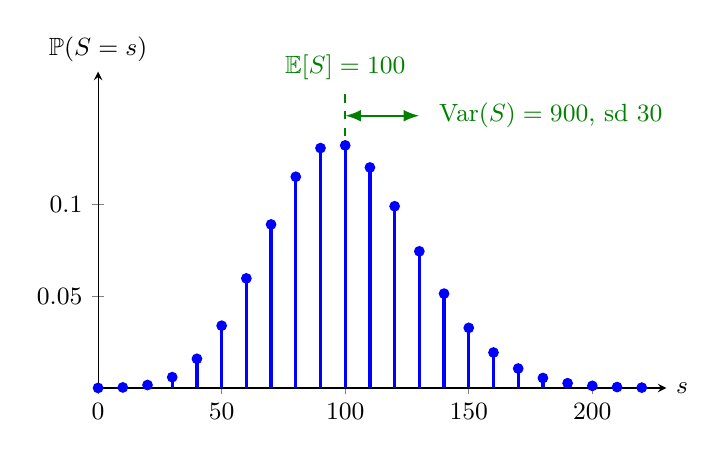
\begin{tikzpicture}[font=\small, >={Latex[length=2mm]}]
  \begin{axis}[
    axis lines=left, xmin=0, xmax=230, ymin=0, ymax=0.172,
    xtick={0,50,100,150,200}, ytick={0.05,0.1},
    yticklabel style={/pgf/number format/fixed},
    xlabel={$s$}, ylabel={$\mathbb P(S=s)$},
    xlabel style={at={(axis description cs:1,0)}, anchor=west},
    ylabel style={rotate=-90, at={(axis description cs:0,1)}, anchor=south},
    width=8.8cm, height=5.6cm, clip=false
    ]
    \addplot[blue, very thick, ycomb, mark=*, mark size=1.3pt] coordinates {
      (0,0.00003) (10,0.00030) (20,0.00162) (30,0.00589) (40,0.01587) (50,0.03387) (60,0.05958)
      (70,0.08890) (80,0.11482) (90,0.13042) (100,0.13187) (110,0.11988) (120,0.09879) (130,0.07430)
      (140,0.05130) (150,0.03268) (160,0.01929) (170,0.01059) (180,0.00543) (190,0.00260) (200,0.00117)
      (210,0.00050) (220,0.00020)};
    \draw[green!50!black, thick, dashed] (axis cs:100,0.137) -- (axis cs:100,0.162);
    \node[green!50!black, anchor=south] at (axis cs:100,0.162) {$\mathbb E[S]=100$};
    \draw[<->, green!50!black, thick] (axis cs:100,0.148) -- (axis cs:130,0.148);
    \node[green!50!black, anchor=west] at (axis cs:134,0.148) {$\operatorname{Var}(S)=900$, sd $30$};
  \end{axis}
\end{tikzpicture}
\end{document}
